\documentclass[]{elsarticle} %review=doublespace preprint=single 5p=2 column
%%% Begin My package additions %%%%%%%%%%%%%%%%%%%
\usepackage[hyphens]{url}



\usepackage{lineno} % add
\providecommand{\tightlist}{%
  \setlength{\itemsep}{0pt}\setlength{\parskip}{0pt}}

\usepackage{graphicx}
\usepackage{booktabs} % book-quality tables
%%%%%%%%%%%%%%%% end my additions to header

\usepackage[T1]{fontenc}
\usepackage{lmodern}
\usepackage{amssymb,amsmath}
\usepackage{ifxetex,ifluatex}
\usepackage{fixltx2e} % provides \textsubscript
% use upquote if available, for straight quotes in verbatim environments
\IfFileExists{upquote.sty}{\usepackage{upquote}}{}
\ifnum 0\ifxetex 1\fi\ifluatex 1\fi=0 % if pdftex
  \usepackage[utf8]{inputenc}
\else % if luatex or xelatex
  \usepackage{fontspec}
  \ifxetex
    \usepackage{xltxtra,xunicode}
  \fi
  \defaultfontfeatures{Mapping=tex-text,Scale=MatchLowercase}
  \newcommand{\euro}{€}
\fi
% use microtype if available
\IfFileExists{microtype.sty}{\usepackage{microtype}}{}
\bibliographystyle{elsarticle-harv}
\usepackage{longtable}
\usepackage{graphicx}
\ifxetex
  \usepackage[setpagesize=false, % page size defined by xetex
              unicode=false, % unicode breaks when used with xetex
              xetex]{hyperref}
\else
  \usepackage[unicode=true]{hyperref}
\fi
\hypersetup{breaklinks=true,
            bookmarks=true,
            pdfauthor={},
            pdftitle={Building Footprint Identification with Airborne LiDAR: A Final Project for FOR 796},
            colorlinks=false,
            urlcolor=blue,
            linkcolor=magenta,
            pdfborder={0 0 0}}
\urlstyle{same}  % don't use monospace font for urls

\setcounter{secnumdepth}{5}
% Pandoc toggle for numbering sections (defaults to be off)

% Pandoc citation processing
\newlength{\cslhangindent}
\setlength{\cslhangindent}{1.5em}
\newlength{\csllabelwidth}
\setlength{\csllabelwidth}{3em}
% for Pandoc 2.8 to 2.10.1
\newenvironment{cslreferences}%
  {}%
  {\par}
% For Pandoc 2.11+
\newenvironment{CSLReferences}[2] % #1 hanging-ident, #2 entry spacing
 {% don't indent paragraphs
  \setlength{\parindent}{0pt}
  % turn on hanging indent if param 1 is 1
  \ifodd #1 \everypar{\setlength{\hangindent}{\cslhangindent}}\ignorespaces\fi
  % set entry spacing
  \ifnum #2 > 0
  \setlength{\parskip}{#2\baselineskip}
  \fi
 }%
 {}
\usepackage{calc}
\newcommand{\CSLBlock}[1]{#1\hfill\break}
\newcommand{\CSLLeftMargin}[1]{\parbox[t]{\csllabelwidth}{#1}}
\newcommand{\CSLRightInline}[1]{\parbox[t]{\linewidth - \csllabelwidth}{#1}\break}
\newcommand{\CSLIndent}[1]{\hspace{\cslhangindent}#1}

% Pandoc header
\usepackage{setspace}\doublespacing
\usepackage{float}
\usepackage{booktabs}
\usepackage{longtable}
\usepackage{array}
\usepackage{multirow}
\usepackage{wrapfig}
\usepackage{float}
\usepackage{colortbl}
\usepackage{pdflscape}
\usepackage{tabu}
\usepackage{threeparttable}
\usepackage{threeparttablex}
\usepackage[normalem]{ulem}
\usepackage{makecell}
\usepackage{xcolor}



\begin{document}
\begin{frontmatter}

  \title{Building Footprint Identification with Airborne LiDAR: A Final Project for FOR 796}
    \author[]{Lucas K Johnson}
  
      
  \begin{abstract}
  This is a test.
  \end{abstract}
  
 \end{frontmatter}

\hypertarget{introduction}{%
\section{Introduction}\label{introduction}}

\hypertarget{methods}{%
\section{Methods}\label{methods}}

\hypertarget{building-and-lidar-data}{%
\subsection{Building and LiDAR Data}\label{building-and-lidar-data}}

Rasterized building footprint data served as the response data in this study
Microsoft (2018).
The raw raster contains counts of the number of buildings intersecting each
pixel.
This data was converted to a Boolean raster where ones represent any buildings
present, and zeroes represent no buildings present.
This data was chosen for it's availability across the entire country, it's high
accuracy (\textgreater{} 99\% positive predictive value; Pourpeikari Heris et al. (2020)), and it's 30m resolution.

The raw LiDAR data originates from a single LiDAR acquisition covering portions
of Erie, Genesee, and Livingston counties in western New York made available
by the New York Stat GIS Program Office (New York Office of Information Technology Services 2019).
The raw LiDAR data was then height-normalized and converted into a set of 39
predictors chosen for their prevalence in models of forest structure
(Hawbaker et al. 2010; Huang et al. 2019; Pflugmacher et al. 2014).
LiDAR data was selected due to it's known ability to characterize three
dimensional height-profiles at high-resolution.
More specifically, these forest-structure predictors were chosen for
practicality.
It would be a great benefit to those mapping forest structure with LiDAR if the
same predictors could also be leveraged for building better forest masks.

The LiDAR predictors, in raster stack form, were overlaid with the Boolean
building raster to create stack of data where each pixel contained a set of 39
predictors and one building indicator response variable.
A stratified random sample was conducted on the raster stack, with the building
indicator providing the levels of stratification.
3,500 observations (pixel locations) were selected from each stratum resulting
in 7,000 observations for model training and testing.
This final dataset was converted to a 7000x40 (rows, columns) data frame.
The lidR (Roussel and Auty 2020; Jean-Romain et al. 2020) and raster (Hijmans 2021) packages were used for
height-normalization and dataset generation.

Additionally, principle components were derived from the final dataset to
remove multicollinearity from the 39 predictors (R Core Team 2021).
This alternative dataset consisted of the first seven principle components,
as they accounted for \(\ge\) 95\% of the information in the predictors.
This alternative dataset was a 7000x7 data frame.

\hypertarget{models}{%
\subsection{Models}\label{models}}

Three candidate classification models were fit to a random 70\%
(calibration data; n =
3500
)
of the observations, with the remaining 30\% reserved for model performance
assessment (holdout data; n =
1500
).

The first candidate model was a simple logistic regression model (R Core Team 2021),
and was trained on the principle components variant of the calibration data.
The second candidate model was a random forest (RF herafter) trained with
the ranger R package (Wright and Ziegler 2017) and the calibration dataset.
The third candidate model was a stochastic gradient boosting machine
(LGB hereafter) trained with the LightGBM R package (Ke et al. 2021)
and the calibration dataset.
The hyperparemeters for both the RF and LGB models were selected using a grid
search where each combination of hyperparameters were compared against eachother
using the cross-entropy loss function (CEL; Equation \eqref{eq:cel})
computed from a random five-fold cross-validation with the calibration dataset.
CEL is computed as follows:

\begin{equation}
\operatorname{CEL} = \sum_{i=1}^{n}{-\log{(\hat{y_{i}})}} \label{eq:cel}
\end{equation}

Where \(n\) is the number of observations in the fold, and \(\hat{y_i}\) is
the predicted probability of the true class.

Each of the models was assessed against the holdout dataset and compared to one
another using overall accuracy, specificity, sensitivity, and AUC.
Additionally ROC curves were plotted for each model's results on the holdout
set.
The caret and pROC R packages were used to compute these accuracy metrics
(Kuhn 2021; Robin et al. 2011).

\hypertarget{results}{%
\section{Results}\label{results}}

The RF model performed the best across all accuray metrics (Table \ref{tab:metrics}).
The LGB model was more specific but less sensitive than the Logisitc
model, and only scored marginally better in AUC and Overall Accuracy.
However, all three candidate models performed quite well with
all AUC values \(\geq\) 0.87, and all overall accuracies \(\geq\) 0.79.
The ROC curves plotted in Figure \ref{fig:roc} display similar patterns.

\begin{table}

\caption{\label{tab:metrics}Model accuracy metrics computed against 30\% holdout partition (n = 1500).}
\centering
\fontsize{12}{14}\selectfont
\begin{tabular}[t]{lrrrr}
\toprule
\multicolumn{1}{c}{Model} & \multicolumn{1}{c}{AUC} & \multicolumn{1}{c}{Overall Accuracy} & \multicolumn{1}{c}{Sensitivity} & \multicolumn{1}{c}{Specificity}\\
\midrule
Logistic & 0.87 & 0.79 & 0.83 & 0.75\\
\addlinespace
LGB & 0.88 & 0.80 & 0.81 & 0.78\\
\addlinespace
RF & 0.96 & 0.90 & 0.92 & 0.89\\
\bottomrule
\end{tabular}
\end{table}

\begin{figure}
\centering
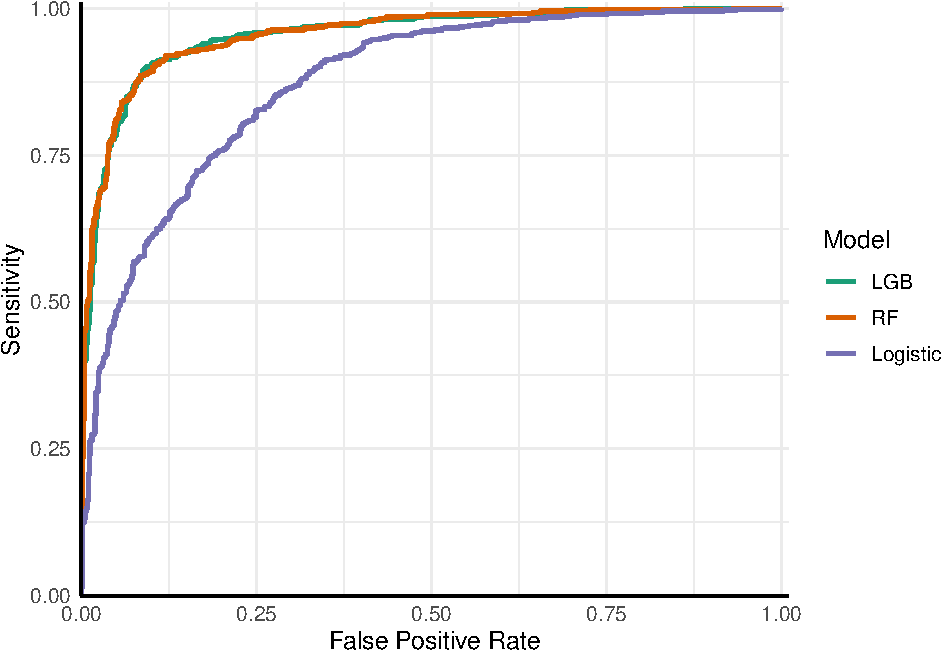
\includegraphics{report_files/figure-latex/roc-1.pdf}
\caption{\label{fig:roc}ROC curves showing sensitivity against specificity for each model.}
\end{figure}

\hypertarget{discussion}{%
\section{Discussion}\label{discussion}}

\begin{itemize}
\item
  RF was superior to all the others
\item
  Logistic still rather good. Makes you wonder if the marginal benefits of ML here
  are worth the effort, time, understandability
\item
  What could have been done better?

  \begin{itemize}
  \tightlist
  \item
    ensembling methods?
  \item
    wider ranges of hyperparameters
  \item
    larger inclusion than just 95\% of the information for principle components
    and logistic regression.
  \item
    Timing. Response from 2018. LiDAR from 2019
  \end{itemize}
\item
  What might these models be used for

  \begin{itemize}
  \tightlist
  \item
    Since the predictors herein are primarily used for predicting forest
    structure - these models make a relatively easy way to extract man-made
    structures away from LiDAR-based maps of forest structure like biomass.
  \item
    There are questions about transferrability of these data from this region
    and this lidar coverages to others from different locations and times.
  \end{itemize}
\end{itemize}

\newpage{}

\hypertarget{references}{%
\section*{References}\label{references}}
\addcontentsline{toc}{section}{References}

\hypertarget{refs}{}
\begin{CSLReferences}{1}{0}
\leavevmode\vadjust pre{\hypertarget{ref-rmd_man}{}}%
Allaire, JJ, Yihui Xie, Jonathan McPherson, Javier Luraschi, Kevin Ushey, Aron Atkins, Hadley Wickham, Joe Cheng, Winston Chang, and Richard Iannone. 2021. \emph{Rmarkdown: Dynamic Documents for r}. \url{https://github.com/rstudio/rmarkdown}.

\leavevmode\vadjust pre{\hypertarget{ref-Hawbaker2010}{}}%
Hawbaker, Todd J., Terje Gobakken, Adrian Lesak, Eric Trømborg, Kirk Contrucci, and Volker Radeloff. 2010. {``{Light Detection and Ranging-Based Measures of Mixed Hardwood Forest Structure}.''} \emph{Forest Science} 56 (3): 313--26. \url{https://doi.org/10.1093/forestscience/56.3.313}.

\leavevmode\vadjust pre{\hypertarget{ref-tidyselect}{}}%
Henry, Lionel, and Hadley Wickham. 2021. \emph{Tidyselect: Select from a Set of Strings}. \url{https://CRAN.R-project.org/package=tidyselect}.

\leavevmode\vadjust pre{\hypertarget{ref-Raster2021}{}}%
Hijmans, Robert J. 2021. \emph{Raster: Geographic Data Analysis and Modeling}. \url{https://CRAN.R-project.org/package=raster}.

\leavevmode\vadjust pre{\hypertarget{ref-Huang2019}{}}%
Huang, Wenli, Katelyn Dolan, Anu Swatantran, Kristofer Johnson, Hao Tang, Jarlath O'Neil-Dunne, Ralph Dubayah, and George Hurtt. 2019. {``High-Resolution Mapping of Aboveground Biomass for Forest Carbon Monitoring System in the Tri-State Region of Maryland, Pennsylvania and Delaware, {USA}.''} \emph{Environmental Research Letters} 14 (9): 095002. \url{https://doi.org/10.1088/1748-9326/ab2917}.

\leavevmode\vadjust pre{\hypertarget{ref-lidrRSE}{}}%
Jean-Romain, Roussel, David Auty, Nicholas C. Coops, Piotr Tompalski, Tristan R. H. Goodbody, Andrew Sánchez Meador, Jean-François Bourdon, Florian de Boissieu, and Alexis Achim. 2020. {``lidR: An r Package for Analysis of Airborne Laser Scanning (ALS) Data.''} \emph{Remote Sensing of Environment} 251: 112061. \url{https://doi.org/10.1016/j.rse.2020.112061}.

\leavevmode\vadjust pre{\hypertarget{ref-Guolin2021}{}}%
Ke, Guolin, Damien Soukhavong, James Lamb, Qi Meng, Thomas Finley, Taifeng Wang, Wei Chen, Weidong Ma, Qiwei Ye, and Tie-Yan Liu. 2021. \emph{Lightgbm: Light Gradient Boosting Machine}. \url{https://CRAN.R-project.org/package=lightgbm}.

\leavevmode\vadjust pre{\hypertarget{ref-caret}{}}%
Kuhn, Max. 2021. \emph{Caret: Classification and Regression Training}. \url{https://CRAN.R-project.org/package=caret}.

\leavevmode\vadjust pre{\hypertarget{ref-Microsoft}{}}%
Microsoft. 2018. {``{US Building Footprints.}''} Microsoft.

\leavevmode\vadjust pre{\hypertarget{ref-EGL_Lidar}{}}%
New York Office of Information Technology Services. 2019. {``{LIDAR collection (QL2) for Erie, Genesee, and Livingston Counties New York Lidar; Classified Point Cloud}.''}

\leavevmode\vadjust pre{\hypertarget{ref-Pflugmacher2014}{}}%
Pflugmacher, Dirk, Warren B. Cohen, Robert E. Kennedy, and Zhiqiang Yang. 2014. {``Using Landsat-Derived Disturbance and Recovery History and Lidar to Map Forest Biomass Dynamics.''} \emph{Remote Sensing of Environment} 151: 124--37. \url{https://doi.org/10.1016/j.rse.2013.05.033}.

\leavevmode\vadjust pre{\hypertarget{ref-Heris2020}{}}%
Pourpeikari Heris, Mehdi, Nathan Foks, Kenneth J Bagstad, and Austin Troy. 2020. {``A National Dataset of Rasterized Building Footprints for the u.s.''} U.S. Geological Survey. \url{https://doi.org/10.5066/P9J2Y1WG}.

\leavevmode\vadjust pre{\hypertarget{ref-RCore}{}}%
R Core Team. 2021. \emph{R: A Language and Environment for Statistical Computing}. Vienna, Austria: R Foundation for Statistical Computing. \url{https://www.R-project.org/}.

\leavevmode\vadjust pre{\hypertarget{ref-pROC}{}}%
Robin, Xavier, Natacha Turck, Alexandre Hainard, Natalia Tiberti, Frédérique Lisacek, Jean-Charles Sanchez, and Markus Müller. 2011. {``pROC: An Open-Source Package for r and s+ to Analyze and Compare ROC Curves.''} \emph{BMC Bioinformatics} 12: 77.

\leavevmode\vadjust pre{\hypertarget{ref-lidrCRAN}{}}%
Roussel, Jean-Romain, and David Auty. 2020. \emph{Airborne LiDAR Data Manipulation and Visualization for Forestry Applications}. \url{https://cran.r-project.org/package=lidR}.

\leavevmode\vadjust pre{\hypertarget{ref-Bing}{}}%
Team, Bing Maps. 2018. {``{Computer Generated Building Footprints for the United States.}''} Microsoft.

\leavevmode\vadjust pre{\hypertarget{ref-ggplot2}{}}%
Wickham, Hadley. 2016. \emph{Ggplot2: Elegant Graphics for Data Analysis}. Springer-Verlag New York. \url{https://ggplot2.tidyverse.org}.

\leavevmode\vadjust pre{\hypertarget{ref-dplyr}{}}%
Wickham, Hadley, Romain François, Lionel Henry, and Kirill Müller. 2021. \emph{Dplyr: A Grammar of Data Manipulation}. \url{https://CRAN.R-project.org/package=dplyr}.

\leavevmode\vadjust pre{\hypertarget{ref-Wright2017}{}}%
Wright, Marvin N., and Andreas Ziegler. 2017. {``Ranger: A Fast Implementation of Random Forests for High Dimensional Data in c++ and r.''} \emph{Journal of Statistical Software, Articles} 77 (1): 1--17. \url{https://doi.org/10.18637/jss.v077.i01}.

\leavevmode\vadjust pre{\hypertarget{ref-rmd_guide}{}}%
Xie, Yihui, J. J. Allaire, and Garrett Grolemund. 2018. \emph{R Markdown: The Definitive Guide}. Boca Raton, Florida: Chapman; Hall/CRC. \url{https://bookdown.org/yihui/rmarkdown}.

\leavevmode\vadjust pre{\hypertarget{ref-rmd_cook}{}}%
Xie, Yihui, Christophe Dervieux, and Emily Riederer. 2020. \emph{R Markdown Cookbook}. Boca Raton, Florida: Chapman; Hall/CRC. \url{https://bookdown.org/yihui/rmarkdown-cookbook}.

\leavevmode\vadjust pre{\hypertarget{ref-kbl}{}}%
Zhu, Hao. 2021. \emph{kableExtra: Construct Complex Table with 'Kable' and Pipe Syntax}.

\end{CSLReferences}


\end{document}
